\begin{spacing}{2}
    \section{研究方法}
\end{spacing}
U-Net首次出现在一次医疗图像分割赛事中。U-Net基于全卷积网路,使用对称结构并且在小数据集表现优异。同时,由于医疗影像的特殊性,作者在论文中特别提到了对于像医疗影像这样的尺寸巨大图像的特殊处理过程。

遥感图像和医疗影像的共同之处在于,数据集小、尺寸巨大。可以说,应用在医疗影像上的U-Net为我们提供了对遥感图像进行分割的重要思路。
\subsection{数据集选择及处理}
这次选择的数据集是Inria Aerial Image Labeling Dataset\cite{maggiori2017dataset}。数据集的图片大小为$5000\times 5000$,共计180组360张3通道遥感图像。样例如图\ref{Fig:sample_dataset}。

\begin{figure}[!t]
		\centering
		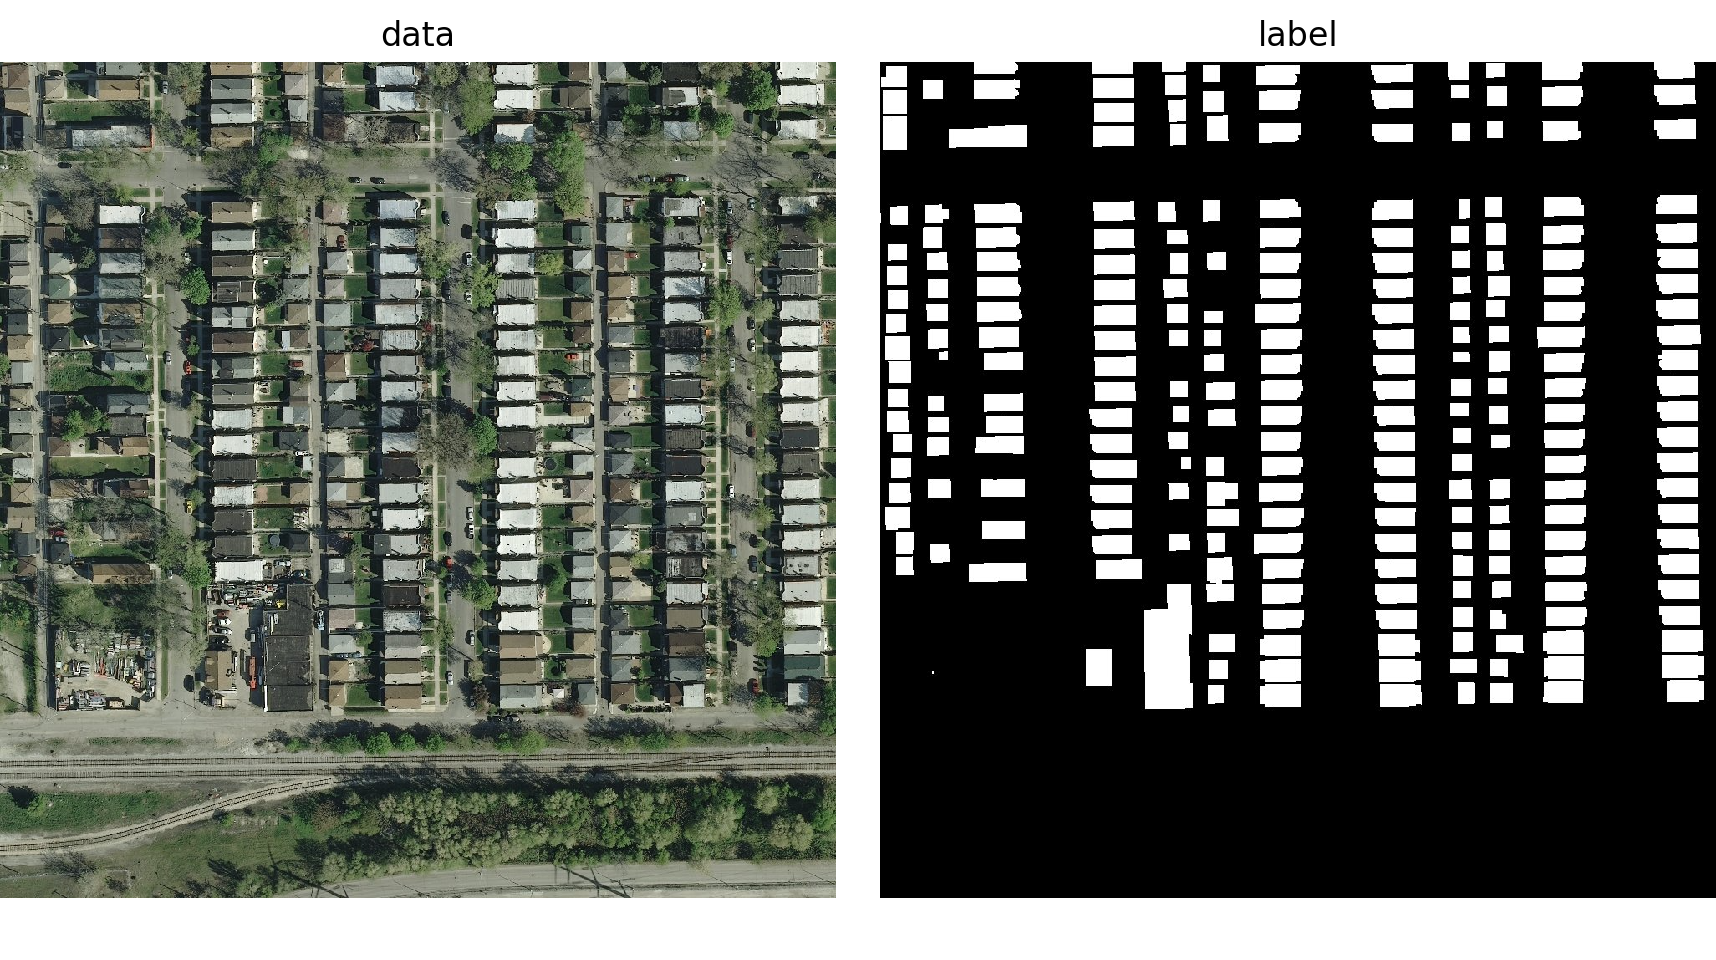
\includegraphics[width=1\textwidth]{Figures/sample_dataset.png}
		\caption{数据集样例图}
		\label{Fig:sample_dataset}
\end{figure}

由于显存限制,经过测试,$500\times 500$左右大小的图片一次只能只能训练一张。如果每次只训练一张的话,会陷入局部最优解。因此将图片切割为$250\times 250$左右大小的图片,mini batch size 大小可以设置为4。

由于池化核的大小为$2\times 2$,因此输入图片的大小最好是2的整次方。最终确定将图片切割为$256\times 256$。原图尺寸大小为$5000\times 5000$,因此将原图调整大小至$4864\times 4864$大小之后再进行分割。这样共得到了64980张图像。由于数据集本身已经够大,因此不再做数据拓展。
\subsection{图像处理流程设计}
\subsubsection{网络结构}
初始的U-Net网络结构如图\ref{Fig:unet_construction}所示。

网络分为收缩路径和扩张路径两部分。在收缩路径中,进行两次卷积核大小为$3\times 3$的卷积之后再进行$2\times 2$的最大池化。在扩张路径中将收缩路径中的卷积层拼接之后再进行两次大小为$3\times 3$的卷积。之后再进行反卷积慢慢恢复到原图像大小。

论文\cite{ronneberger2015u}中使用valid卷积方式。但是经过计算,$256\times 256$大小的图片在通过U-Net网络后,输出图片大小为$68\times 68$,与原图像大小相差太大,因此在这里选用same卷积方式,这样输出图片大小仍为$256\times 256$。除此之外没有对U-Net做更多结构上的修改。
\begin{figure}[!t]
    \centering
    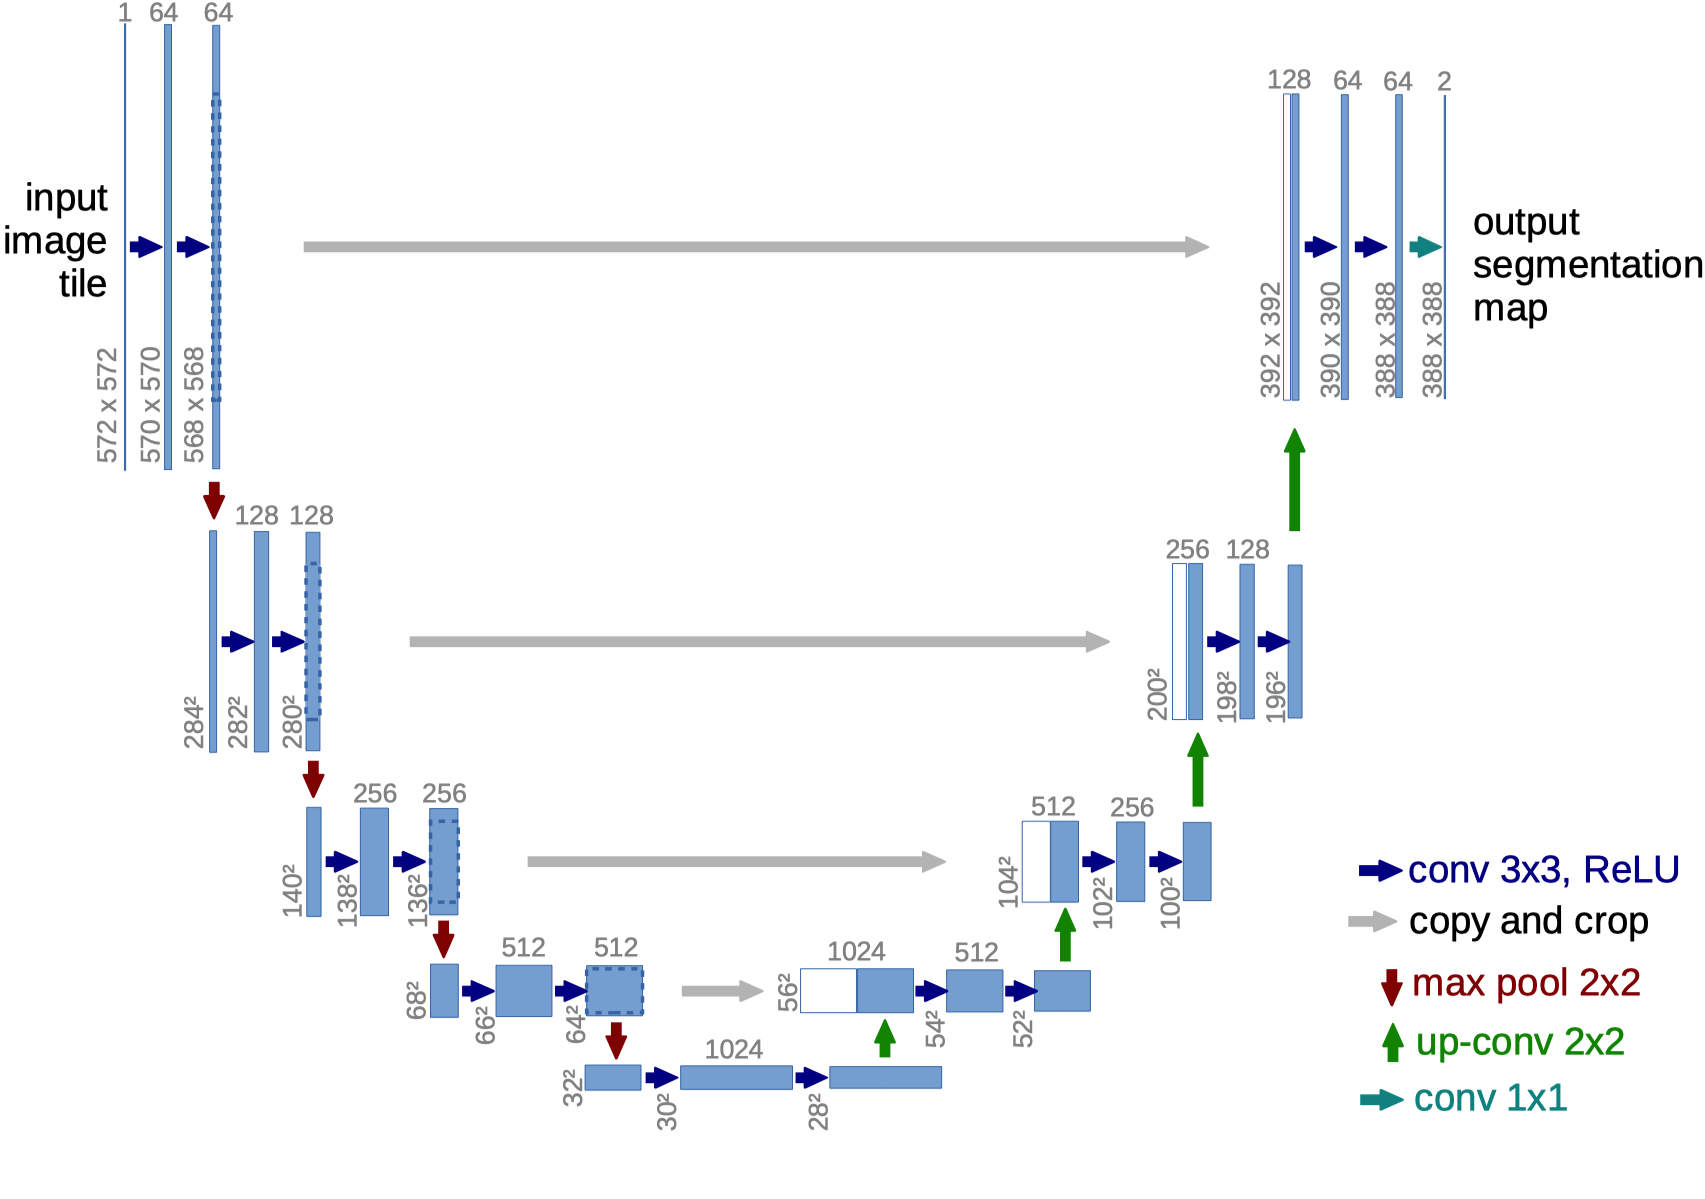
\includegraphics[width=1\textwidth]{Figures/unet_construction.png}
    \caption{U-Net网络结构(来源\cite{ronneberger2015u})}
    \label{Fig:unet_construction}
\end{figure}
\subsubsection{实验后处理}
通过之后的损失函数中权重的不同,训练出几个参数不同的神经网络。将同一张图通过不同的神经网络之后得到的输出图进行像素级或操作,得到融合的生成图。再对得到输出图之后对图像进行形态学处理,去除小面积空洞图和小面积误报区。
% https://blog.csdn.net/traumland/article/details/51419963
考虑到房屋多为多边形,因此使用霍夫变换检测出输出图中的多边形并标注为房屋。

在之前的论文中有人使用条件随机场对生成的图片做更精准的切分,这里时间有限就没有做这种尝试。
\subsection{损失设计}
原始的U-Net网络论文中使用的是交叉熵加上一些正则化项。除了交叉熵之外,此次实验还设计另外两种损失函数,将在之后的实验中做出对比。

在下面这三种损失函数中,都先对卷积网络输出图像做了soft-max计算:
\begin{equation}\label{softmax}
p_k(x)=\exp(\frac{a_k(x)}{\sum\limits_{k'=1}^K \ \exp(a_{k'}(x))})
\end{equation}

公式\ref{softmax}中$K$是分割类别数,$k\in K$。具体到这个数据集来说,类别分为建筑和非建筑,因此$K=2$。

$\mathbb{Z}^2$为全体像素集合,$x\in \mathbb{Z}^2$。$a_k(x)$即在$x$处类别$k$的取值。
\subsubsection{带权重的交叉熵}
\begin{equation}\label{entropy}
E=\sum_{x\in \Omega}\ w(x)\cdot \log(p_{l(x)}(x))
\end{equation}

公式\ref{entropy}中$l: \Omega\rightarrow\{1,\cdots,K\}$是每个像素点真正的类别;$w: \Omega\rightarrow\mathbb{R}$是权重。该权重将取不同值,在训练过程中进行比较。
\subsubsection{类别平衡交叉熵}
\begin{equation}\label{class_balanced_cross_entropy}
    l=-\beta\cdot \sum\limits_{j\in Y_+}\ \log\ \Pr(y_j=1|X)-(1-\beta)\cdot \sum\limits_{j\in Y_-}\ \log\ \Pr(y_j=0|X)
\end{equation}

在\cite{xie2015holistically}中提出了一种被称为类别平衡交叉熵函数的方法计算损失。因为边缘像素的数量远远小于非边缘像素的数量,因此在训练时容易陷入向全取非边缘像素方向的局部最优。在遥感图像中,被标记为房屋的像素与非房屋的像素数量也不是十分均衡的,因此在这里尝试使用类比平衡交叉熵,防止陷入局部最优解。

公式\ref{class_balanced_cross_entropy}中引入了一个像素级的类别平衡权重$\beta$,其值是被标记为建筑的像素占所有像素的比值。这实际上也是一种带权重的交叉熵,只不过该交叉熵的权重取得是两种标签的比值。

